% !TEX TS-program = pdflatex
% !TEX encoding = UTF-8 Unicode

% This is a simple template for a LaTeX document using the "article" class.
% See "book", "report", "letter" for other types of document.

\documentclass[10pt,twocolumn]{article}

\usepackage[utf8]{inputenc} % set input encoding (not needed with XeLaTeX)
\usepackage{geometry} 
\usepackage{graphicx}
\usepackage{listings} 
\usepackage{caption} 
\usepackage{xcolor,colortbl}
\usepackage{mathtools}
\usepackage{amsfonts}
\usepackage{amssymb}
\usepackage{amsthm}
\usepackage{subfig}
\usepackage{wrapfig}
\usepackage{tabularx}
\usepackage{pdflscape}

\graphicspath{ {images/} }

%%% Examples of Article customizations
% These packages are optional, depending whether you want the features they provide.
% See the LaTeX Companion or other references for full information.

%%% PAGE DIMENSIONS
% to change the page dimensions
\geometry{a4paper} % or letterpaper (US) or a5paper or....
\geometry{margin=0.55in} % for example, change the margins to 2 inches all round
% \geometry{landscape} % set up the page for landscape
%   read geometry.pdf for detailed page layout information

% \usepackage[parfill]{parskip} % Activate to begin paragraphs with an empty line rather than an indent

%%% PACKAGES
\usepackage{booktabs} % for much better looking tables
\usepackage{array} % for better arrays (eg matrices) in maths
\usepackage{paralist} % very flexible & customisable lists (eg. enumerate/itemize, etc.)
\usepackage{verbatim} % adds environment for commenting out blocks of text & for better verbatim
\usepackage{subfig} % make it possible to include more than one captioned figure/table in a single float
\usepackage{indentfirst}
% These packages are all incorporated in the memoir class to one degree or another...

%%% HEADERS & FOOTERS
\usepackage{fancyhdr} % This should be set AFTER setting up the page geometry
\pagestyle{fancy} % options: empty , plain , fancy
\renewcommand{\headrulewidth}{0pt} % customise the layout...
\lhead{}\chead{}\rhead{}
\lfoot{}\cfoot{\thepage}\rfoot{}

%%% SECTION TITLE APPEARANCE
\usepackage{sectsty}
\allsectionsfont{\sffamily\mdseries\upshape} % (See the fntguide.pdf for font help)
% (This matches ConTeXt defaults)

%%% ToC (table of contents) APPEARANCE
\usepackage[nottoc,notlof,notlot]{tocbibind} % Put the bibliography in the ToC
\usepackage[titles,subfigure]{tocloft} % Alter the style of the Table of Contents
\renewcommand{\cftsecfont}{\rmfamily\mdseries\upshape}
\renewcommand{\cftsecpagefont}{\rmfamily\mdseries\upshape} % No bold!
\setlength{\parindent}{0.5cm} 

\newcommand{\subsubfloat}[2]{%
  \begin{tabular}{@{}c@{}}#1\\#2\end{tabular}%
}

%%% END Article customizations

%%% The "real" document content comes below...

\title{On 2D and 3D Shapes Based On Primality Tests}
\author{Marcin Barylski}
\date{\small{Created: May 7, 2017 \\ The last update: June 9, 2019}}

\definecolor{Gray}{gray}{0.85}
\definecolor{LightCyan}{rgb}{0.88,1,1}
\newcolumntype{a}{>{\columncolor{Gray}}c}
\newcolumntype{b}{>{\columncolor{white}}c}

\begin{document}
\maketitle

\begin{abstract}
Based on primality property change for two consecutive terms of infinite sequence of natural numbers it is possible to establish rules which allow to draw a figure. This work is devoted to studies on various sequences of natural numbers which produced interesting 2D and 3D outputs.
\end{abstract}


\section{Introduction}

Each natural number $n$ belongs to either prime (P) or non-prime (NP) set. If we arrange $N$ natural numbers $n_1$, $n_2$, ... $n_N$ in an ordered sequence $S$ ($S(i)$ = $n_i$), then we can create a corresponding ordered sequence $P$ of $N$ boolean values ($P(i)$ is either $True$ or $False$, 1 $\leq$ i $\leq$ N) based on primality of $n_i$. $P(i)$ is $True$ if $S(i)$ is prime, otherwise is $False$. For instance, if $S = 1, 2, 3, 4, 5, 6$ then $P = False, True, True, False, True, False$. \par
Observation of changes in $P$ provides information about changeability of primality property in $S$. If $S(i)$ is prime and $S(i+1)$ is not prime, then $P(i)$ = $True$ and $P(i+1)$ = $False$ (change from $True$ to $False$).  If $S(i)$ is not prime and $S(i+1)$ is prime, then $P(i)$ = $False$ and $P(i+1)$ = $True$ (change from $False$ to $True$). We can establish yet another sequence $Q$ which indicates primality property change between two consecutive terms of $S$. If $P(i)$ XOR $P(i+1)$ = $True$, then $Q(i+1)$ = $True$, otherwise $Q(i+1)$ = $False$. For instance, if $S = 1, 2, 3, 4, 5, 6$ then $P = False, True, True, False, True, False$ and $Q = N/A, True, False, True, True, True$. For simplication in calculations we can assume that $Q(0)$ will be always $False$.\par

\section{Basic plotting rules}

Values recorded in $Q$ may be used to draw 2D shape. \#Q = \#S , thus shape would have as many points as terms in $S$. We start plotting from point $W$ = $(0, 0)$ and with vector $D$ = $(+1,0)$, which is indicating current direction for next point to be drawn.
If $Q(i)$ XOR $Q(i+1)$ = $False$, then we continue plotting in already established direction. If $Q(i)$ XOR $Q(i+1)$ = $True$, then we change direction (for instance, clockwise: Table $\ref{tablevectorchange}$) before plotting the next point.

\begin{table}[h]
\centering
\caption{Clockwise change of two-dimensional $D$}
\label{tablevectorchange}
\begin{tabular}{|c|c|}
  \hline 
  \rowcolor{LightCyan}
   Initial $D$ (x,y) & New $D$ (x,y) \\
  \hline 
  (0,1) & (-1,0) \\
  \hline 
  (1,0) & (0,1) \\
  \hline 
  (0,-1) & (1,0) \\
  \hline 
  (-1,0) & (0,-1) \\
  \hline 
\end{tabular} 
\end{table}

Plotting algorithm $A$ for 2D figures is depicted in Listing 1. Figure drawing starts from point (0,0) with direction (+1,0). In its main part $A$ is testing primality of elements in $S$, one-by-one, and stores results in $P$. Then (based on difference between two consecutive terms of $P$) $A$ decides on the next point location and draws a single point. Entire operation is repeated until end of $S$ is reached.

\lstset{language=Python}
\lstset{breaklines=true}
\lstset{frame=shadowbox}
\lstset{caption={Plotting algorithm for 2D shape}}
\label{listingplottingbasics}
\begin{lstlisting}[linewidth=8.7cm]
# initial values
W = (0, 0)
D = (+1,0)
P[0] = False

# assuming that S contains N elements
# is_prime(n) returns True iff n is prime
i = 1
for n in S:
   P[i] = is_prime(n)
   # change direction if Q is changing
   if P[i-1] XOR P[i]:
      D = change_direction (D)   
   W += D
   plot_point (W)
   i += 1

def change_direction (D)
   D = rotate_vector_clockwise (D)
   return D

def plot_point (W)
   plot (W.x, W.y, color)
\end{lstlisting}

 In case of 3D plotting, third dimension is added which is changing delta of $z$ (table $\ref{tablevectorchange3d}$ shows rules for such change).

\begin{table}[h]
\centering
\caption{Change of dimension $z$ in three-dimensional $D$}
\label{tablevectorchange3d}
\begin{tabular}{|c|c|}
  \hline 
  \rowcolor{LightCyan}
   Initial $z$ & New $z$ \\
  \hline 
  0 & 1 \\
  \hline 
  1 & -1 \\
  \hline 
  -1 & 0 \\
  \hline 
\end{tabular} 
\end{table}

\section{Advanced plotting rules and metrics}

Basic plotting rules may be suplemented with more advanced rules like points aging, more demanding rules for changing $D$, including changeable length of $D$ and using more than one color to plot the points. \par
Point aging may be defined in a way that each visible point $P_i$ is associated with watchdog $W_i$ which is started when $P_i$ is created. $W_i$ initial value is set to value $AGE_{max}$ ($AGE_{max}$ \textgreater 0) and is decreased by 1 with every iteration if actual point $P_j$ is different than $P_i$. $W_i$ is reset to $AGE_{max}$ if $P_j$ = $P_i$. $P_i$ is removed (aged out) if $W_i$ = $AGE_{min}$ = 0. \par
If point aging is in use, point $P_i$ color selection may be based on $W_i$ value (the bigger value of $W_i$, the hotter color). Color may be also based on total number of hits (the more hits, the hotter color) which is ideal for case without point aging. \par
Each shape can be accompanied with a set of metrics which can be used to compare them and quantify properties in time. Table $\ref{tablemetrics}$ shows such sample metrics.

\begin{table}[h]
\centering
\caption{Metrics}
\label{tablemetrics}
\begin{tabular}{|l|l|}
  \hline 
  \rowcolor{LightCyan}
   Metric & Description\\
  \hline 
  $M_1$: \% of primes &  primes / all $\times$ 100\% \\
  \hline 
  $M_2$: \% of non-primes &  non-primes / all $\times$ 100\%\\
  \hline 
  $M_3$: Max diff in p.X & max(p.X) - min(p.X) \\
  \hline 
  $M_4$: Max diff in p.Y & max(p.Y) - min(p.Y) \\
  \hline 
  $M_5$: Max diff in p.Z & max(p.Z) - min(p.Z) \\
  \hline 
  $M_6$: 2D fill in \% & pts / ($M_3$ $\times$ $M_4$) $\times$ 100\% \\
  \hline 
  $M_7$: 3D fill in \% & pts / ($M_3$ $\times$ $M_4$ $\times$ $M_5$) $\times$ 100\% \\
  \hline 
\end{tabular} 
\end{table}

\section{Results of experiments}

During experiments (which were targeted to find interesting relations and visualisations between primes and composite numbers) various sequences $S_i$ were evaluated (Table $\ref{tablesequences}$).

\begin{table}[h]
\centering
\caption{Sequences $S_i$ subjected to experiments}
\label{tablesequences}
\begin{tabular}{|c|c|}
  \hline 
  \rowcolor{LightCyan}
   i & Formula for $S_i(n)$\\
  \hline 
  1 & 2$\times$n + 1 \\
  \hline 
  2 & 6$\times$n + 1 \\
  \hline 
  3 & 6$\times$n - 1 \\
  \hline 
  4 & 6$\times$n + 1 for n even \\ & 6$\times$n - 1 for n odd \\
  \hline 
  5 & n \\
  \hline 
  6 & 30$\times$n + 1 \\
  \hline 
  7 & 30$\times$n - 1 \\
  \hline 
  8 & 30$\times$n + 1 for n even \\ & 30$\times$n - 1 for n odd \\
  \hline
  9 & sum of decimal digits of n \\
  \hline 
  10 & 1 for n even \\ & 2 for n odd \\
  \hline 
  11 & $\left \lfloor{10 \times sin(n)}\right \rfloor$ \\
  \hline
  12 & random (2, 3, 4, 5, 6, 7, 8, 9) \\
  \hline
\end{tabular} 
\end{table}

Figures 1 and 2 present 2D shapes for $S_i$ (Table $\ref{tablesequences}$) and figures 3 and 4 - corresponding 3D shapes. Experiments were run for the first $10^6$ terms of $S_i$.

\onecolumn

\begin{figure}
\centering

\subfloat{
  \begin{minipage}{\columnwidth}\footnotesize
  \centering

  \subsubfloat{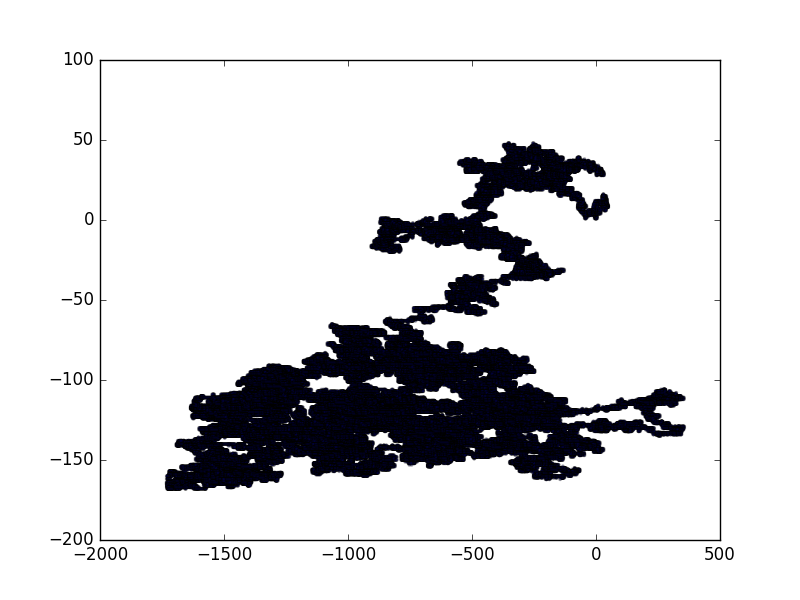
\includegraphics[width=0.45\columnwidth]{f_shape_1}}{$S_1$}
  \qquad
  \subsubfloat{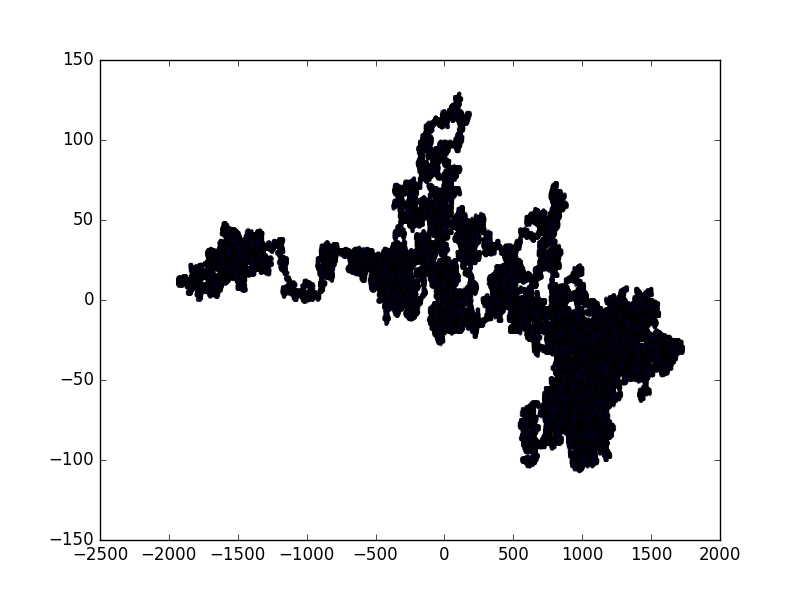
\includegraphics[width=0.45\columnwidth]{f_shape_2}}{$S_2$}
  \qquad
  \subsubfloat{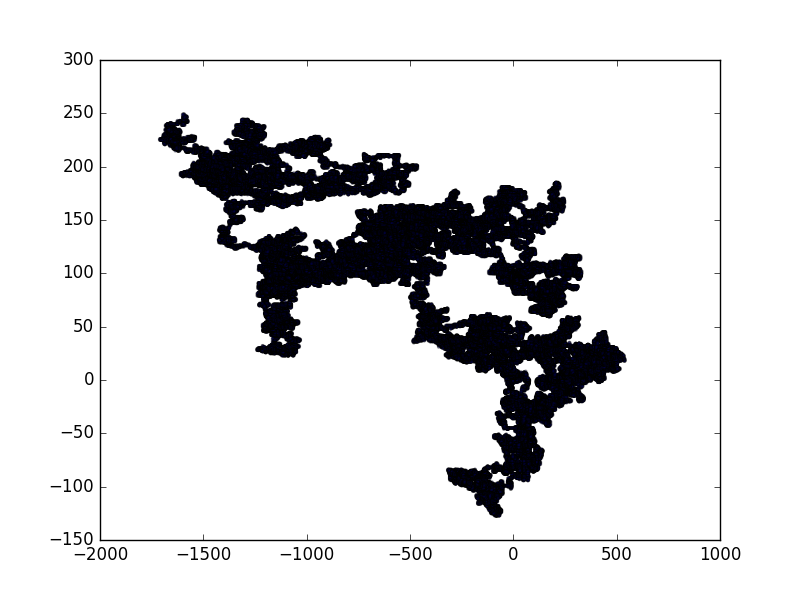
\includegraphics[width=0.45\columnwidth]{f_shape_3}}{$S_3$}
  \qquad
  \subsubfloat{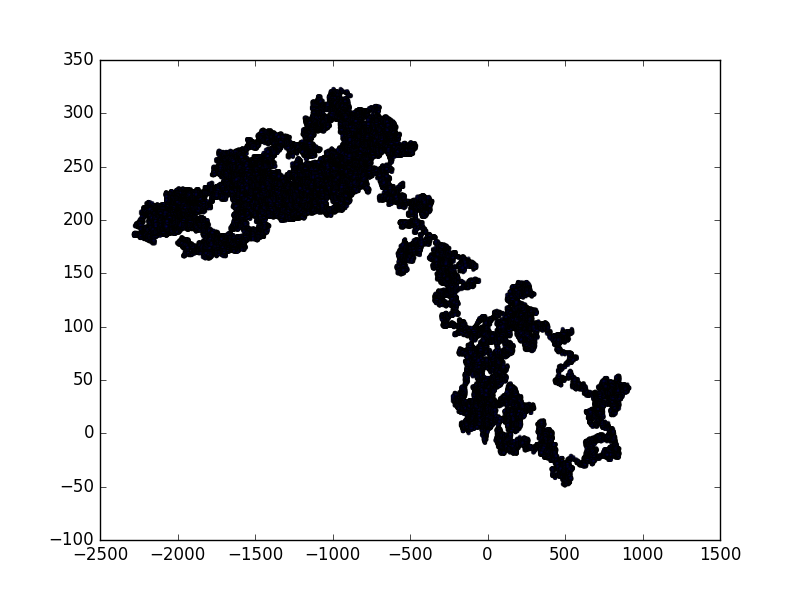
\includegraphics[width=0.45\columnwidth]{f_shape_4}}{$S_4$}
  \qquad
  \subsubfloat{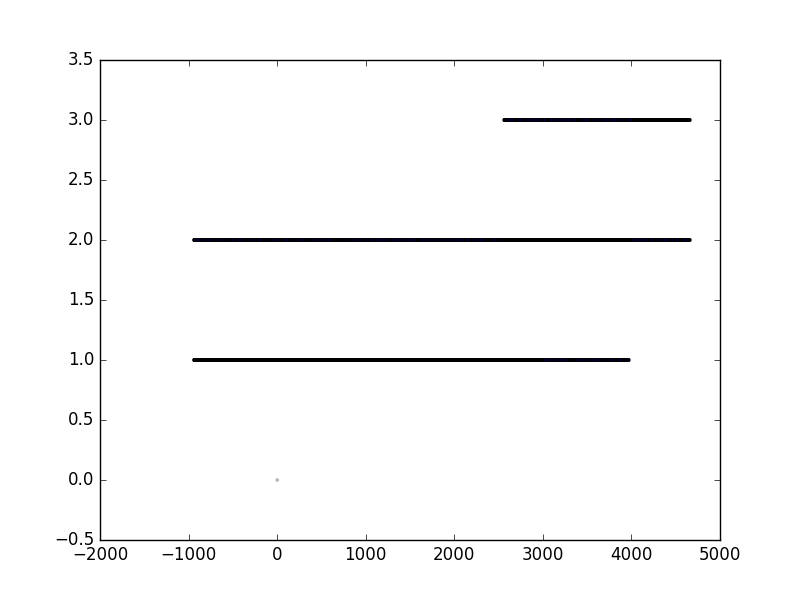
\includegraphics[width=0.45\columnwidth]{f_shape_5}}{$S_5$}
  \qquad
  \subsubfloat{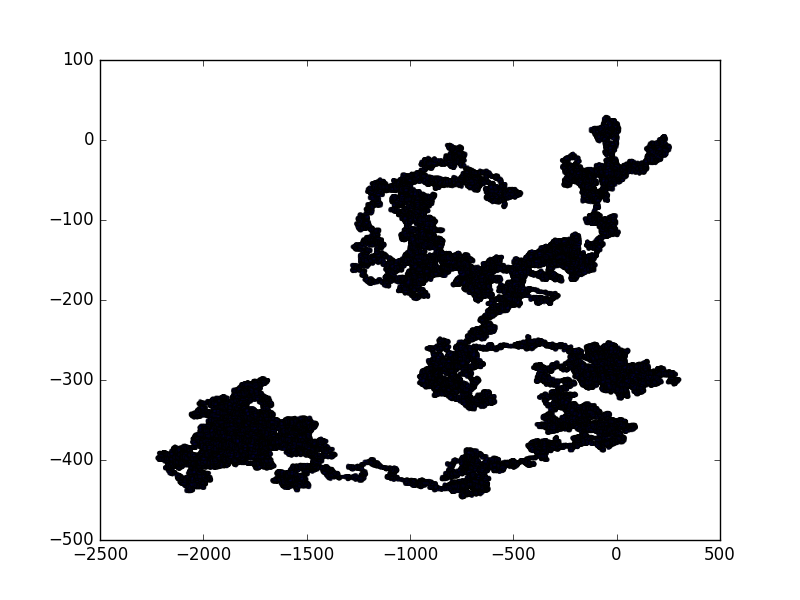
\includegraphics[width=0.45\columnwidth]{f_shape_6}}{$S_6$}
  \qquad
  \subsubfloat{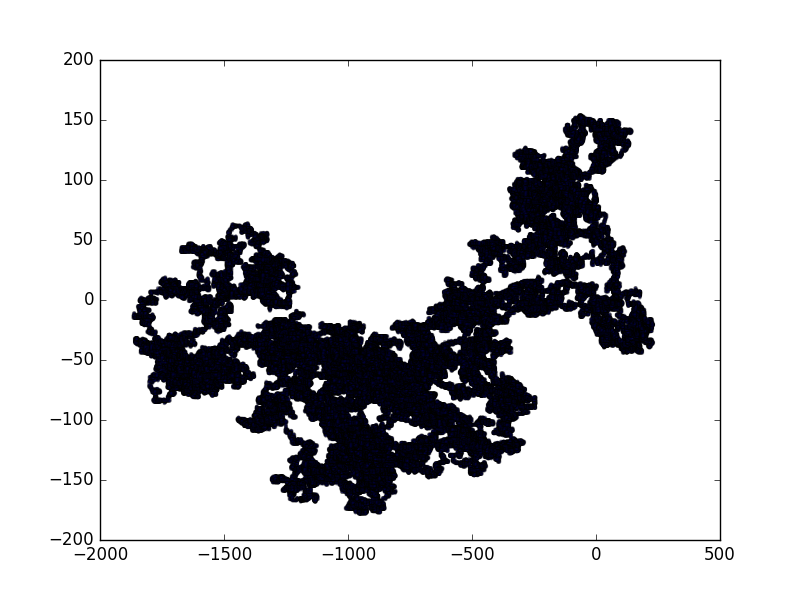
\includegraphics[width=0.45\columnwidth]{f_shape_7}}{$S_7$}
  \qquad
  \subsubfloat{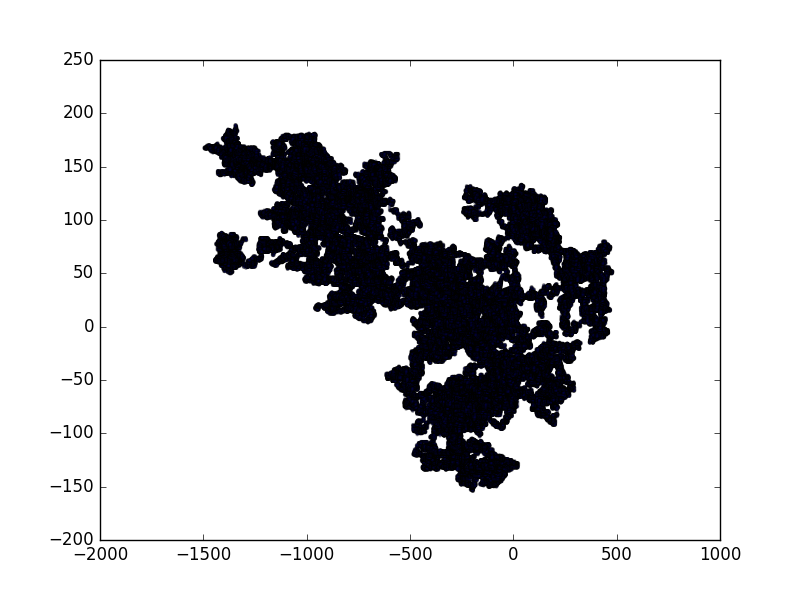
\includegraphics[width=0.45\columnwidth]{f_shape_8}}{$S_8$}

  \end{minipage}
}

\caption{2D plots - sequences 1-8}
\end{figure}

\begin{figure}
\centering

\subfloat{
  \begin{minipage}{\columnwidth}\footnotesize
  \centering

  \subsubfloat{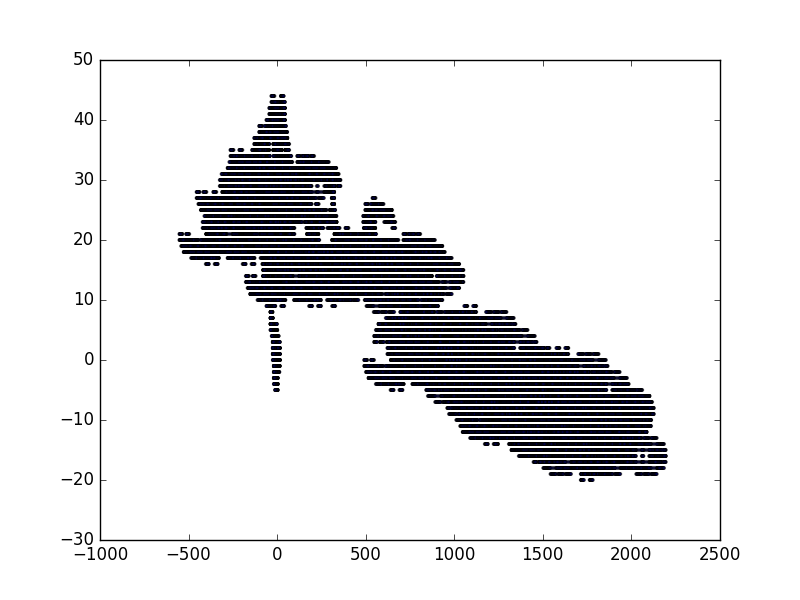
\includegraphics[width=0.40\columnwidth]{f_shape_9}}{$S_9$}
  \qquad
  \subsubfloat{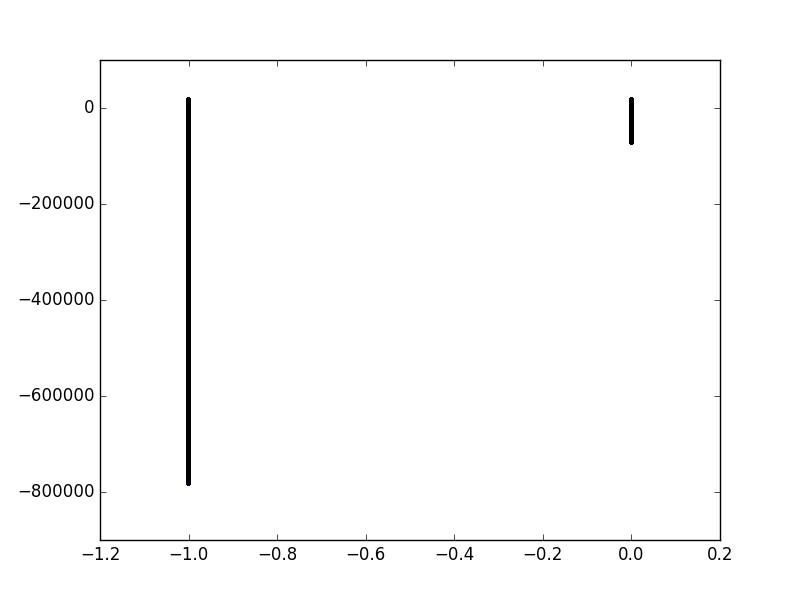
\includegraphics[width=0.40\columnwidth]{f_shape_10}}{$S_{10}$}
  \qquad
  \subsubfloat{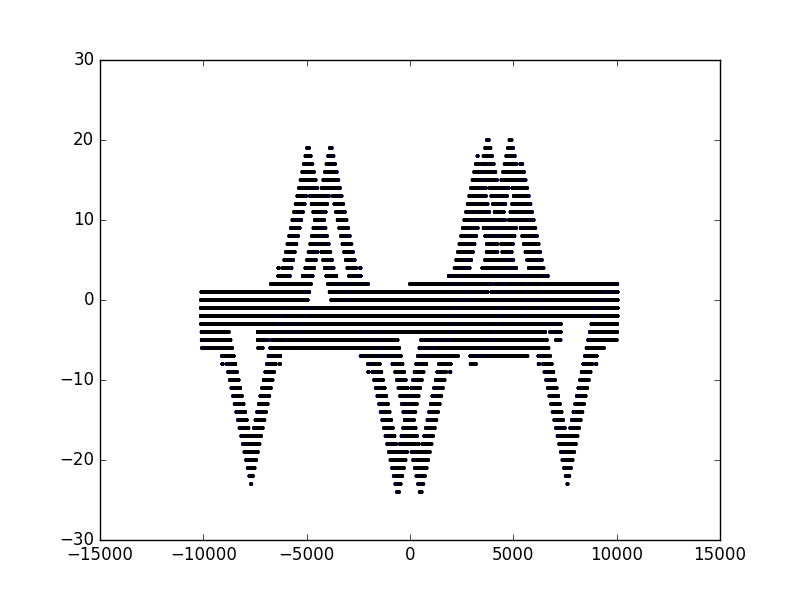
\includegraphics[width=0.40\columnwidth]{f_shape_11}}{$S_{11}$}
  \qquad
  \subsubfloat{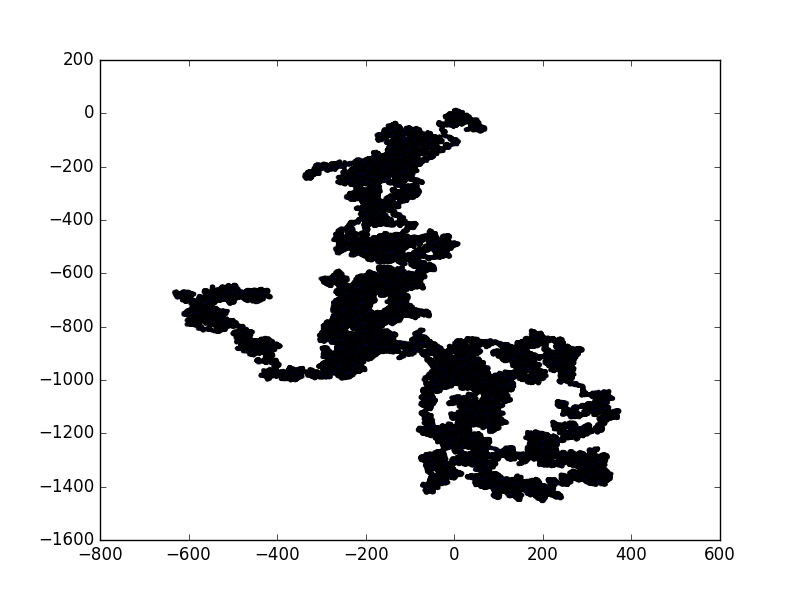
\includegraphics[width=0.40\columnwidth]{f_shape_12}}{$S_{12}$}

  \end{minipage}
}

\caption{2D plots - sequences 9-12}
\end{figure}

\begin{figure}
\centering

\subfloat{
  \begin{minipage}{\columnwidth}\footnotesize
  \centering

  \subsubfloat{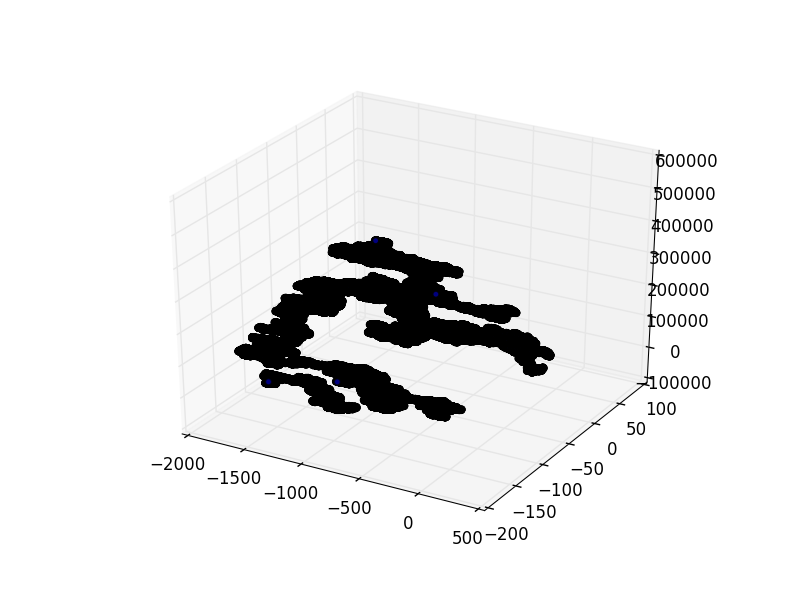
\includegraphics[width=0.45\columnwidth]{f_shape_13d}}{$S_{1}$}
  \qquad
  \subsubfloat{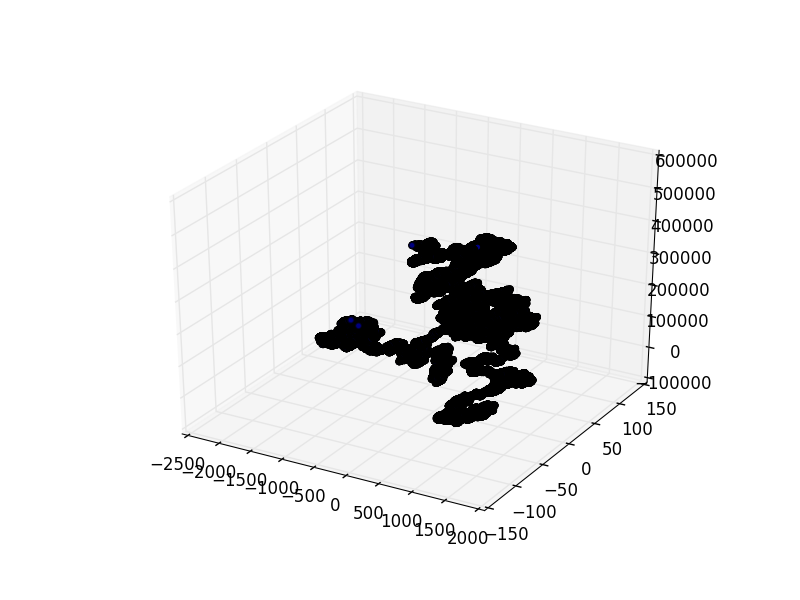
\includegraphics[width=0.45\columnwidth]{f_shape_23d}}{$S_{2}$}
  \qquad
  \subsubfloat{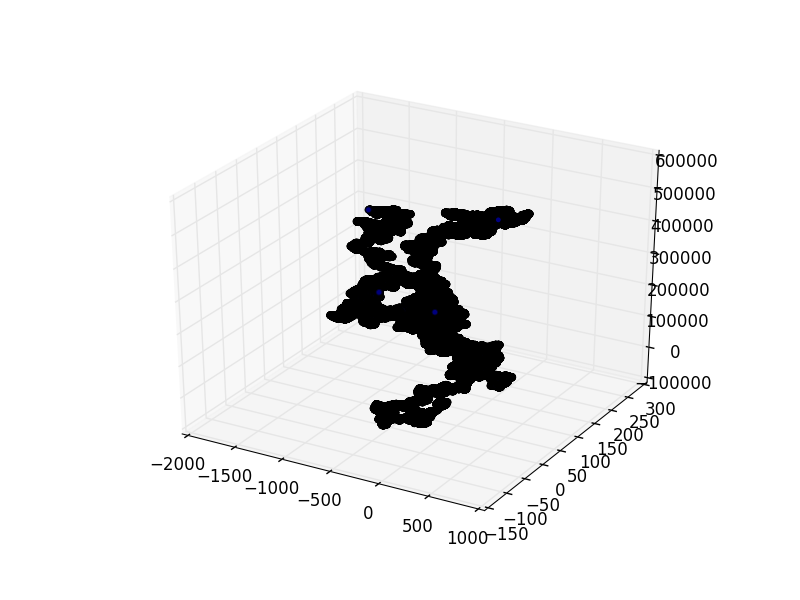
\includegraphics[width=0.45\columnwidth]{f_shape_33d}}{$S_{3}$}
  \qquad
  \subsubfloat{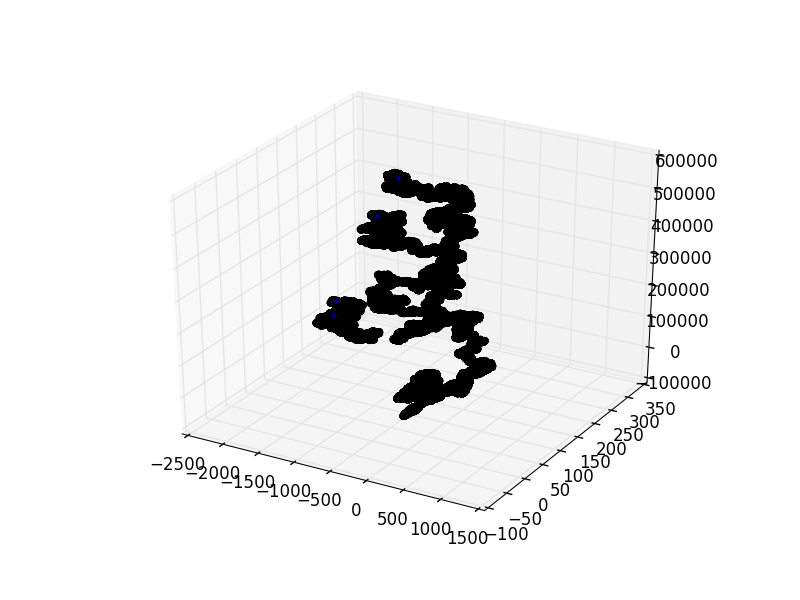
\includegraphics[width=0.45\columnwidth]{f_shape_43d}}{$S_{4}$}

  \end{minipage}
}

\caption{3D plots - sequences 1-4}
\end{figure}

\begin{figure}
\centering

\subfloat{
  \begin{minipage}{\columnwidth}\footnotesize
  \centering

  \subsubfloat{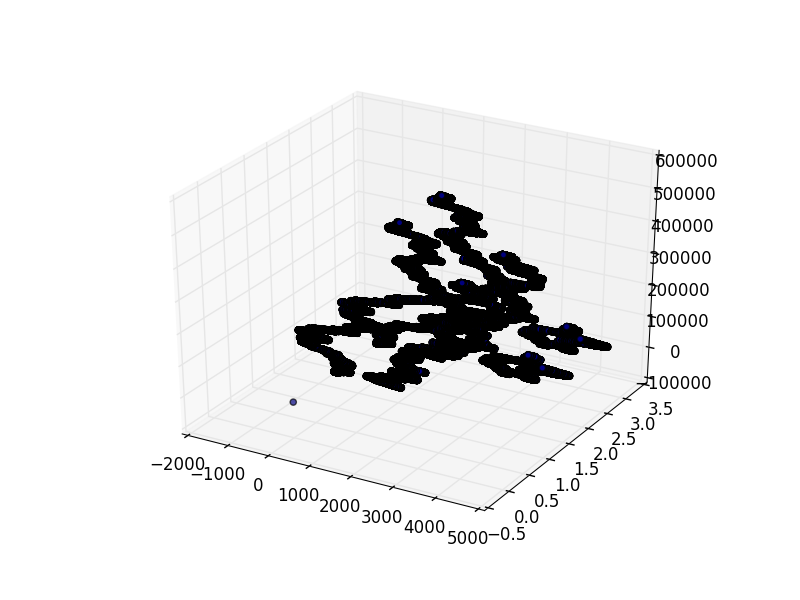
\includegraphics[width=0.45\columnwidth]{f_shape_53d}}{$S_{5}$}
  \qquad
  \subsubfloat{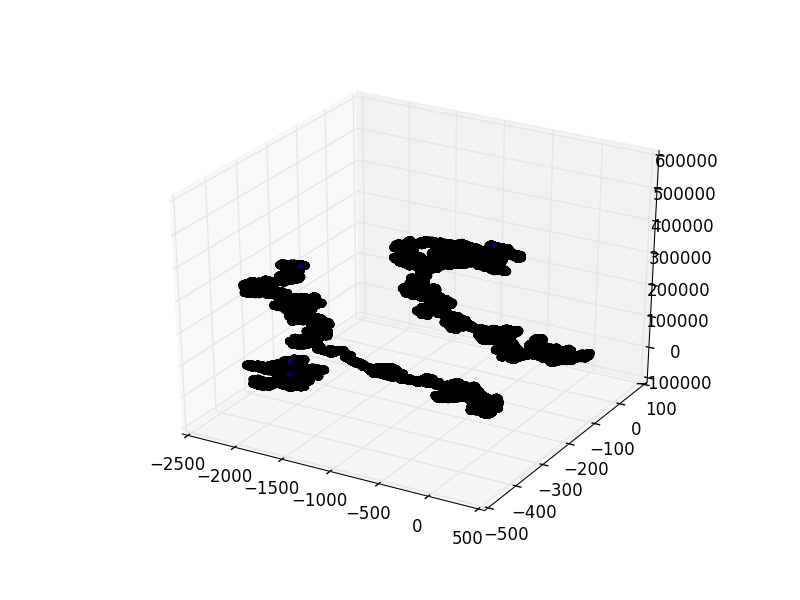
\includegraphics[width=0.45\columnwidth]{f_shape_63d}}{$S_{6}$}
  \qquad
  \subsubfloat{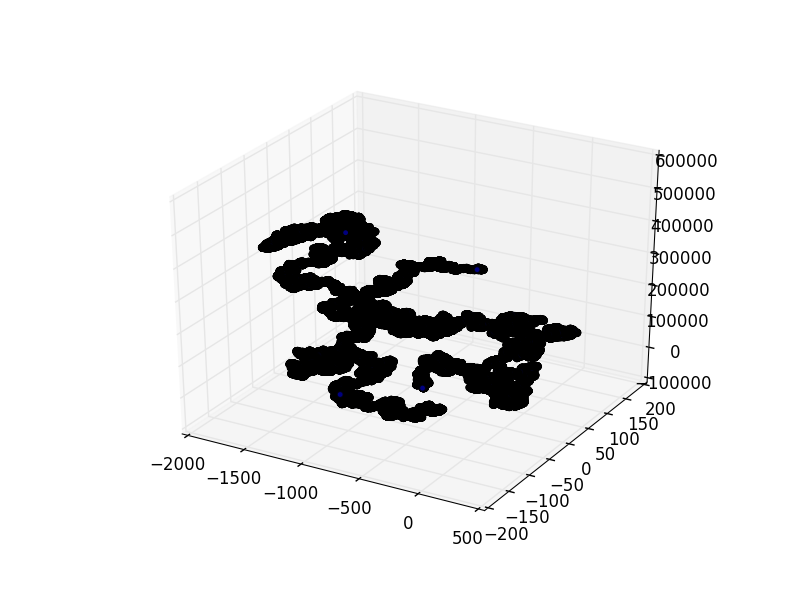
\includegraphics[width=0.45\columnwidth]{f_shape_73d}}{$S_{7}$}
  \qquad
  \subsubfloat{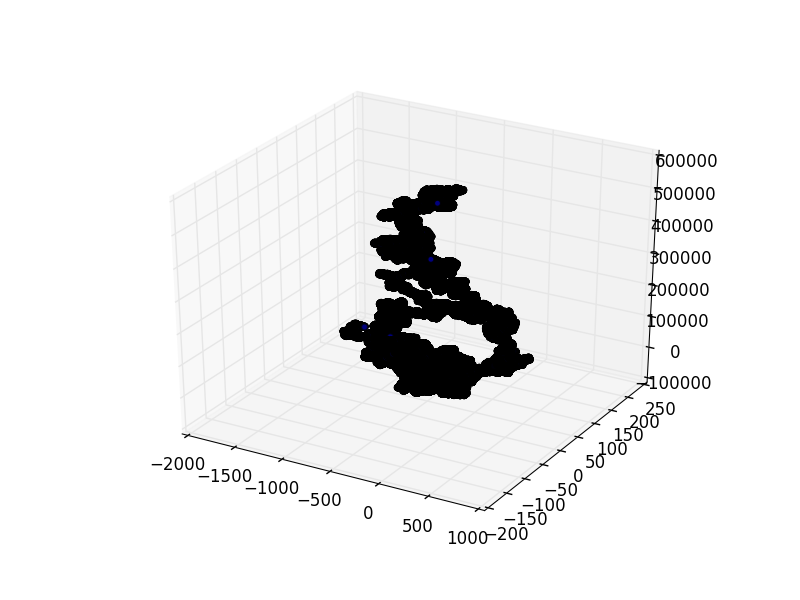
\includegraphics[width=0.45\columnwidth]{f_shape_83d}}{$S_{8}$}
  \qquad
  \subsubfloat{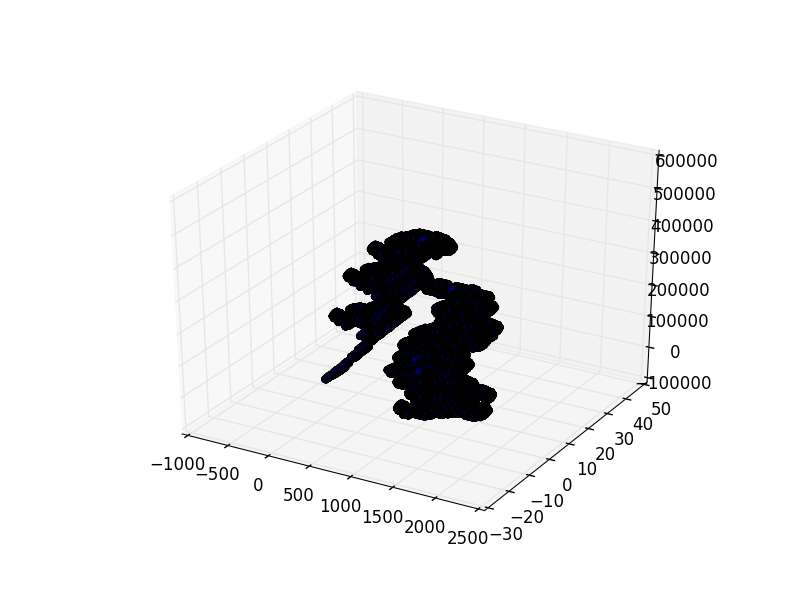
\includegraphics[width=0.45\columnwidth]{f_shape_93d}}{$S_{9}$}
  \qquad
  \subsubfloat{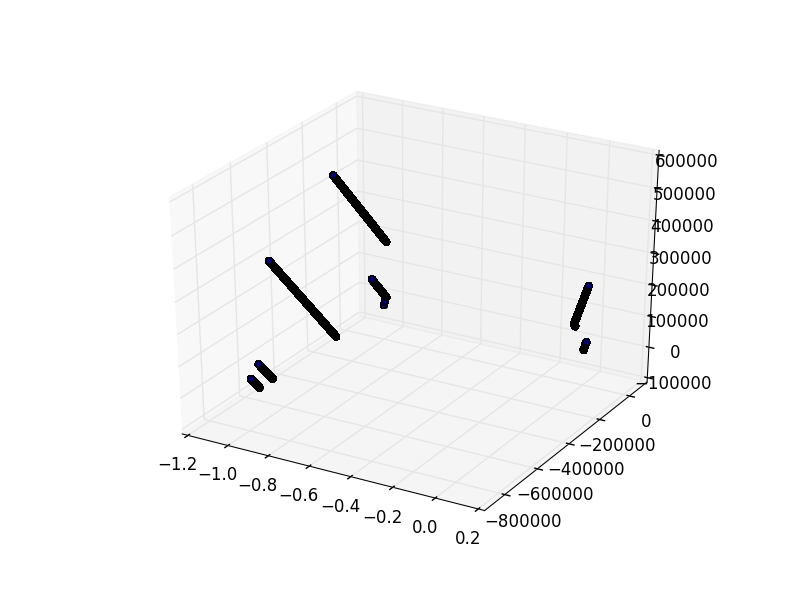
\includegraphics[width=0.45\columnwidth]{f_shape_103d}}{$S_{10}$}
  \qquad
  \subsubfloat{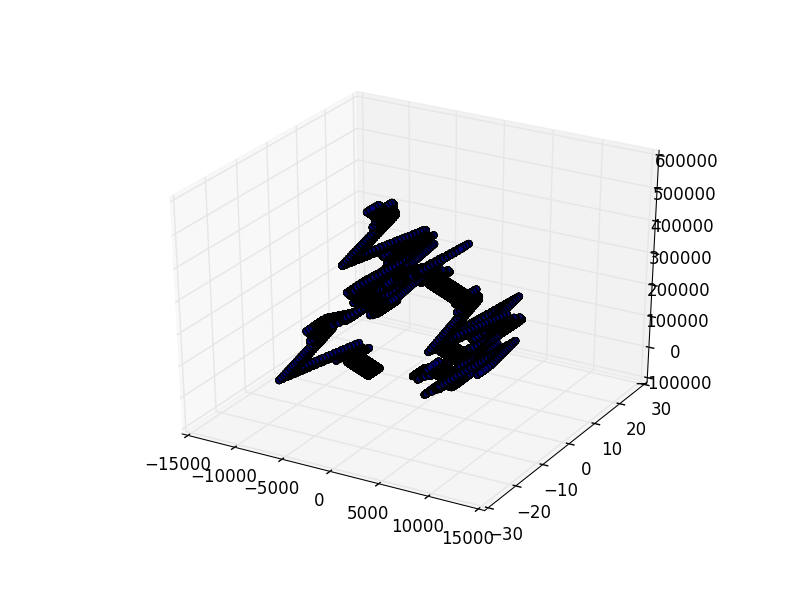
\includegraphics[width=0.45\columnwidth]{f_shape_113d}}{$S_{11}$}
  \qquad
  \subsubfloat{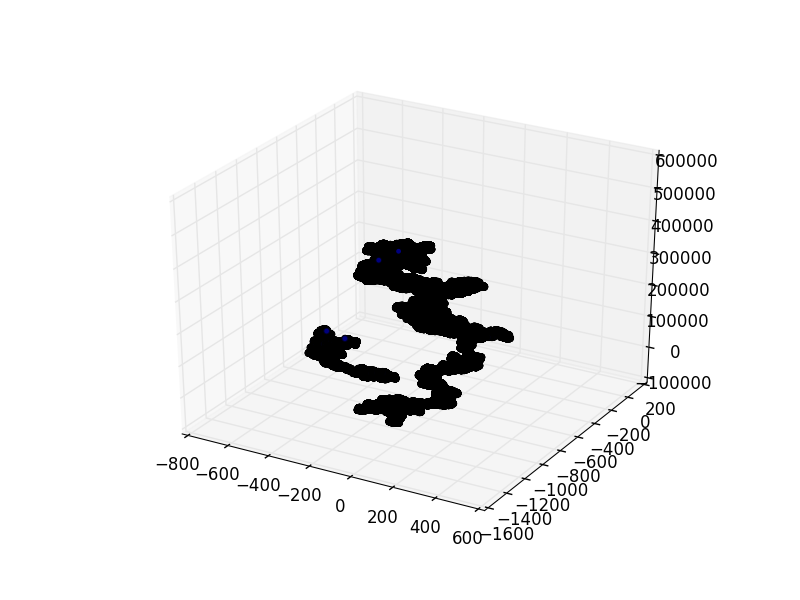
\includegraphics[width=0.45\columnwidth]{f_shape_123d}}{$S_{12}$}

  \end{minipage}
}

\caption{3D plots - sequences 5-12}
\end{figure}

\twocolumn

TBD

\section{Summary and future work}

TBD

\begin{thebibliography}{9}

\bibitem{github}
  \emph{Prime shapes automated generation framework.}
  https://github.com/mbarylsk/prime-shapes/

\end{thebibliography}

\end{document}
